

\begin{figure}[H]
  \centering
  \begin{minipage}[b]{0.45\textwidth}
    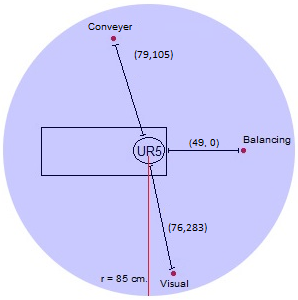
\includegraphics[width=\textwidth]{Design/workcell_1_polar.png}
    \label{fig:position}
  \end{minipage}
  \hfill
  \begin{minipage}[b]{0.45\textwidth}
    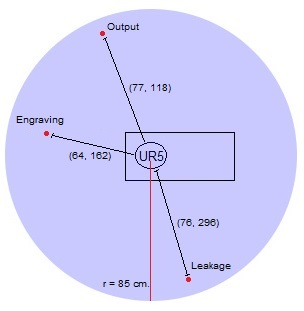
\includegraphics[width=\textwidth]{Design/polar.jpg}  
    \label{fig:velocity}
  \end{minipage}
  {Work-cell first and second part ,with polar coordinates and reach to suited the reach of the UR 5.}
\end{figure}
%Flowchart 1:
\begin{tikzpicture}[node distance=2cm]

%Primary nodes:
\node (start) [startstop] {Rotor arrives on conveyer/queue table};
\node (dec1) [decision, below of=start, yshift=-2.5cm] {Has this rotor been balance tested?};
\node (dec2) [decision, right of=dec1, xshift=3.2cm] {Is the balancing
machine empty?};
\node (pro1) [process, right of=dec2, xshift=3.1cm] {Move the rotor to balancing machine};
\node (out1) [io, below of=pro1, yshift=-3cm] {Balancing complete};
\node (dec3) [decision, below of=dec1, yshift=-6cm] {Has this rotor been visually inspected?};
\node (dec4) [decision, right of=dec3, xshift=3.2cm] {Is visual inspection available?};
\node (pro2) [process, right of=dec4, xshift=3.1cm] {Move the rotor to visual inspection};
\node (out2) [io, below of=pro2, yshift=-3cm] {Visual inspection complete};
\node (stop) [startstop, below of=dec3, yshift=-5cm] {Move rotor to queue table};

%Primary arrows:
\draw [arrow] (start) -- (dec1);
\draw [arrow] (dec1) -- node[anchor=south] {no} (dec2);
\draw [arrow] (dec1) -- node[anchor=west] {yes} (dec3);
\draw [arrow] (dec2) -- node[anchor=south] {yes} (pro1);
\draw [arrow] (pro1) -- (out1);
\draw [arrow] (dec3) -- node[anchor=south] {no} (dec4);
\draw [arrow] (dec3) -- node[anchor=west]  {yes} (stop);
\draw [arrow] (dec4) -- node[anchor=south] {yes} (pro2);
\draw [arrow] (pro2) -- (out2);

%dec2, dec4 -> start:
\node (gui1) [Guidebox, left of=pro1, xshift=-11cm] {};
\node (gui2) [Guidebox, below of=gui1, yshift=-0.85cm] {};
\node (gui6) [Guidebox, left of=pro2, xshift=-11cm] {};
\node (gui7) [Guidebox, below of=gui6, yshift=-0.85cm] {};

%Below dec2:
\node (gui3) [Guidebox, right of=gui2, xshift=5.9cm] {};
\node (gui4) [Guidebox, below of=gui3, yshift=1.9cm] {};
\node (gui5) [Guidebox, right of=gui3, xshift=-1.9cm] {};
\draw [arrow] (dec2) -- node[anchor=west] {no} (gui4);
\draw [arrow] (gui5) -- (gui2);

%Below dec4:
\node (gui8) [Guidebox, right of=gui7, xshift=5.9cm] {};
\node (gui9) [Guidebox, below of=gui8, yshift=1.9cm] {};
\node (gui10) [Guidebox, right of=gui8, xshift=-1.9cm] {};
\draw [arrow] (dec4) -- node[anchor=west] {no} (gui9);

%Line to start:
\node (gui11) [Guidebox, above of=gui1, yshift=2.55cm] {};
\node (gui12) [Guidebox, above of=gui11, yshift=-1.9cm] {};
\node (gui13) [Guidebox, left of=gui11, xshift=1.9cm] {};
\node (gui16) [Guidebox, below of=gui7, yshift=1.9cm] {};
\node (gui17) [Guidebox, left of=gui7, xshift=1.9cm] {};
\draw [arrow] (gui10) -- (gui17);
\draw [arrow] (gui16) -- (gui12);
\draw [arrow] (gui13) -- (start);

%out1, out2 -> dec3, stop:
\node (gui14) [Guidebox, above of=dec3, yshift=1cm] {};
\draw [arrow] (out1) -- (gui14);
\node (gui15) [Guidebox, above of=stop, yshift=-0cm] {};
\draw [arrow] (out2) -- (gui15);

\label{fig:first-part}
\end{tikzpicture}



%Flowchart 2:
\begin{tikzpicture}[node distance=2cm]

%Primary nodes:
\node (start) [startstop] {Rotor arrives on queue-table};
\node (dec1) [decision, below of=start, yshift=-2.5cm] {Has this rotor been leak tested?};
\node (dec2) [decision, right of=dec1, xshift=3.2cm] {Is the leak testing
machine empty?};
\node (pro1) [process, right of=dec2, xshift=3.1cm] {Move the rotor to leak testing machine};
\node (out1) [io, below of=pro1, yshift=-3cm] {Leak testing complete};
\node (dec3) [decision, below of=dec1, yshift=-6cm] {Has this rotor been engraved?};
\node (dec4) [decision, right of=dec3, xshift=3.2cm] {Is the engraving
machine empty?};
\node (pro2) [process, right of=dec4, xshift=3.1cm] {Move the rotor to engraving machine};
\node (out2) [io, below of=pro2, yshift=-3cm] {Engraving complete};
\node (stop) [startstop, below of=dec3, yshift=-5cm] {Move rotor to output pallet};

%Primary arrows:
\draw [arrow] (start) -- (dec1);
\draw [arrow] (dec1) -- node[anchor=south] {no} (dec2);
\draw [arrow] (dec1) -- node[anchor=west] {yes} (dec3);
\draw [arrow] (dec2) -- node[anchor=south] {yes} (pro1);
\draw [arrow] (pro1) -- (out1);
\draw [arrow] (dec3) -- node[anchor=south] {no} (dec4);
\draw [arrow] (dec3) -- node[anchor=west]  {yes} (stop);
\draw [arrow] (dec4) -- node[anchor=south] {yes} (pro2);
\draw [arrow] (pro2) -- (out2);

%dec2, dec4 -> start:
\node (gui1) [Guidebox, left of=pro1, xshift=-11cm] {};
\node (gui2) [Guidebox, below of=gui1, yshift=-0.85cm] {};
\node (gui6) [Guidebox, left of=pro2, xshift=-11cm] {};
\node (gui7) [Guidebox, below of=gui6, yshift=-0.85cm] {};

%Below dec2:
\node (gui3) [Guidebox, right of=gui2, xshift=5.9cm] {};
\node (gui4) [Guidebox, below of=gui3, yshift=1.9cm] {};
\node (gui5) [Guidebox, right of=gui3, xshift=-1.9cm] {};
\draw [arrow] (dec2) -- node[anchor=west] {no} (gui4);
\draw [arrow] (gui5) -- (gui2);

%Below dec4:
\node (gui8) [Guidebox, right of=gui7, xshift=5.9cm] {};
\node (gui9) [Guidebox, below of=gui8, yshift=1.9cm] {};
\node (gui10) [Guidebox, right of=gui8, xshift=-1.9cm] {};
\draw [arrow] (dec4) -- node[anchor=west] {no} (gui9);

%Line to start:
\node (gui11) [Guidebox, above of=gui1, yshift=2.55cm] {};
\node (gui12) [Guidebox, above of=gui11, yshift=-1.9cm] {};
\node (gui13) [Guidebox, left of=gui11, xshift=1.9cm] {};
\node (gui16) [Guidebox, below of=gui7, yshift=1.9cm] {};
\node (gui17) [Guidebox, left of=gui7, xshift=1.9cm] {};
\draw [arrow] (gui10) -- (gui17);
\draw [arrow] (gui16) -- (gui12);
\draw [arrow] (gui13) -- (start);

%out1, out2 -> dec3, stop:
\node (gui14) [Guidebox, above of=dec3, yshift=1cm] {};
\draw [arrow] (out1) -- (gui14);
\node (gui15) [Guidebox, above of=stop, yshift=-0cm] {};
\draw [arrow] (out2) -- (gui15);


\end{tikzpicture}




